\section{Introduction}
Autoregressive Large Language Models (LLMs) have achieved significant success and are widely utilized across diverse natural language processing applications, including dialogue systems~\cite{yi2024survey}, document summarization~\cite{laban2023summedits}, and code generation~\cite{gu2023llm}.
The widespread deployments of LLMs have propelled the development of their capacities to process extended sequences. For instance, GPT supports sequences up to 128K~\cite{achiam2023gpt}, Claude3 up to 200K~\cite{anthropic2024claude}, and Gemini-Pro-1.5~\cite{reid2024gemini} up to 2M tokens.
However, this growth in token length introduces significant challenges, particularly the rapid expansion of cache size during inference. For an 8B LLM, handling a single sequence of 2M tokens can require up to 256GB of cache, severely impacting both GPU memory efficiency and computational runtime efficiency.

In particular, the inference process, for each multi-head self-attention layer, consists of two phases: \textit{prefilling} and \textit{decoding}. In the prefilling phase, LLMs compute and store all Key-Value (KV) cache elements for the tokens in the input prompt.
In the decoding phase, the model autoregressively uses the most recently generated token to retrieve information from the stored cache, producing the next output iteratively.
The large KV cache size introduces two important efficiency challenges: First, it severely affects GPU memory efficiency, making it increasingly difficult to scale with longer inputs. Second, during decoding, increased I/O latency duo to cache access results in substantial delays, degrading runtime efficiency.







To address the challenges posed by large KV cache sizes, various cache eviction methods have been developed~\cite{FastGen,H2o,PyramidInfer,PyramidKV,SnapKV}.
These methods constrain the cache size to a predefined budget by retaining only a subset of elements in each attention head and evicting the rest.
They reduces memory usage and accelerate decoding, facilitating efficient long-sequence inference.
Most of these methods rely on a Top-$k$ selection based on attention weights, to identify and prioritize critical cache elements, deciding which to retain and which to evict.




\begin{figure}[t]  
	
	
	\vspace{-0.2cm}
	\begin{subfigure}[b]{0.45\linewidth}
		\centering
		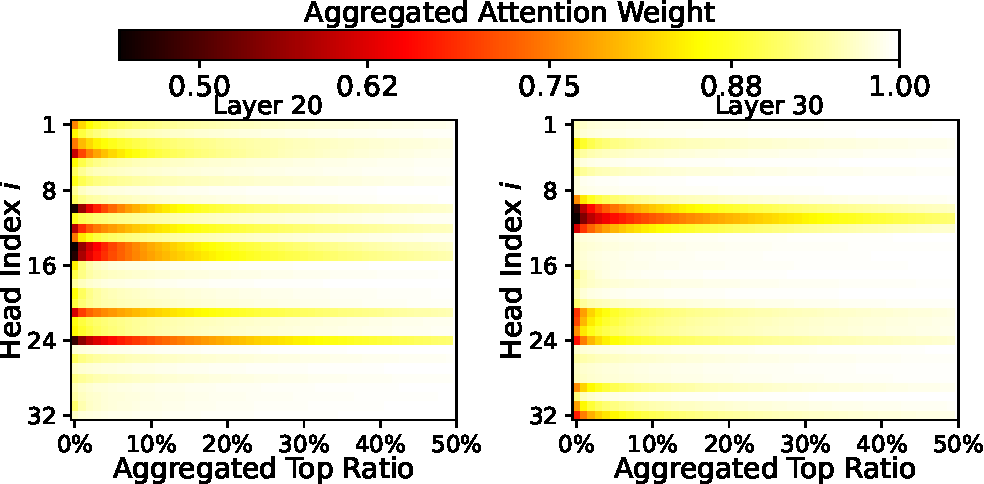
\includegraphics[width=\linewidth]{./Figures/cusum_weight_three_layers.pdf}
		\vspace{-0.4cm}
		\caption{ Varied Attention Concentration Across Heads. }
		\label{fig:accu_weights}  
	\end{subfigure}
	\begin{subfigure}[b]{0.53\linewidth}
		\centering
		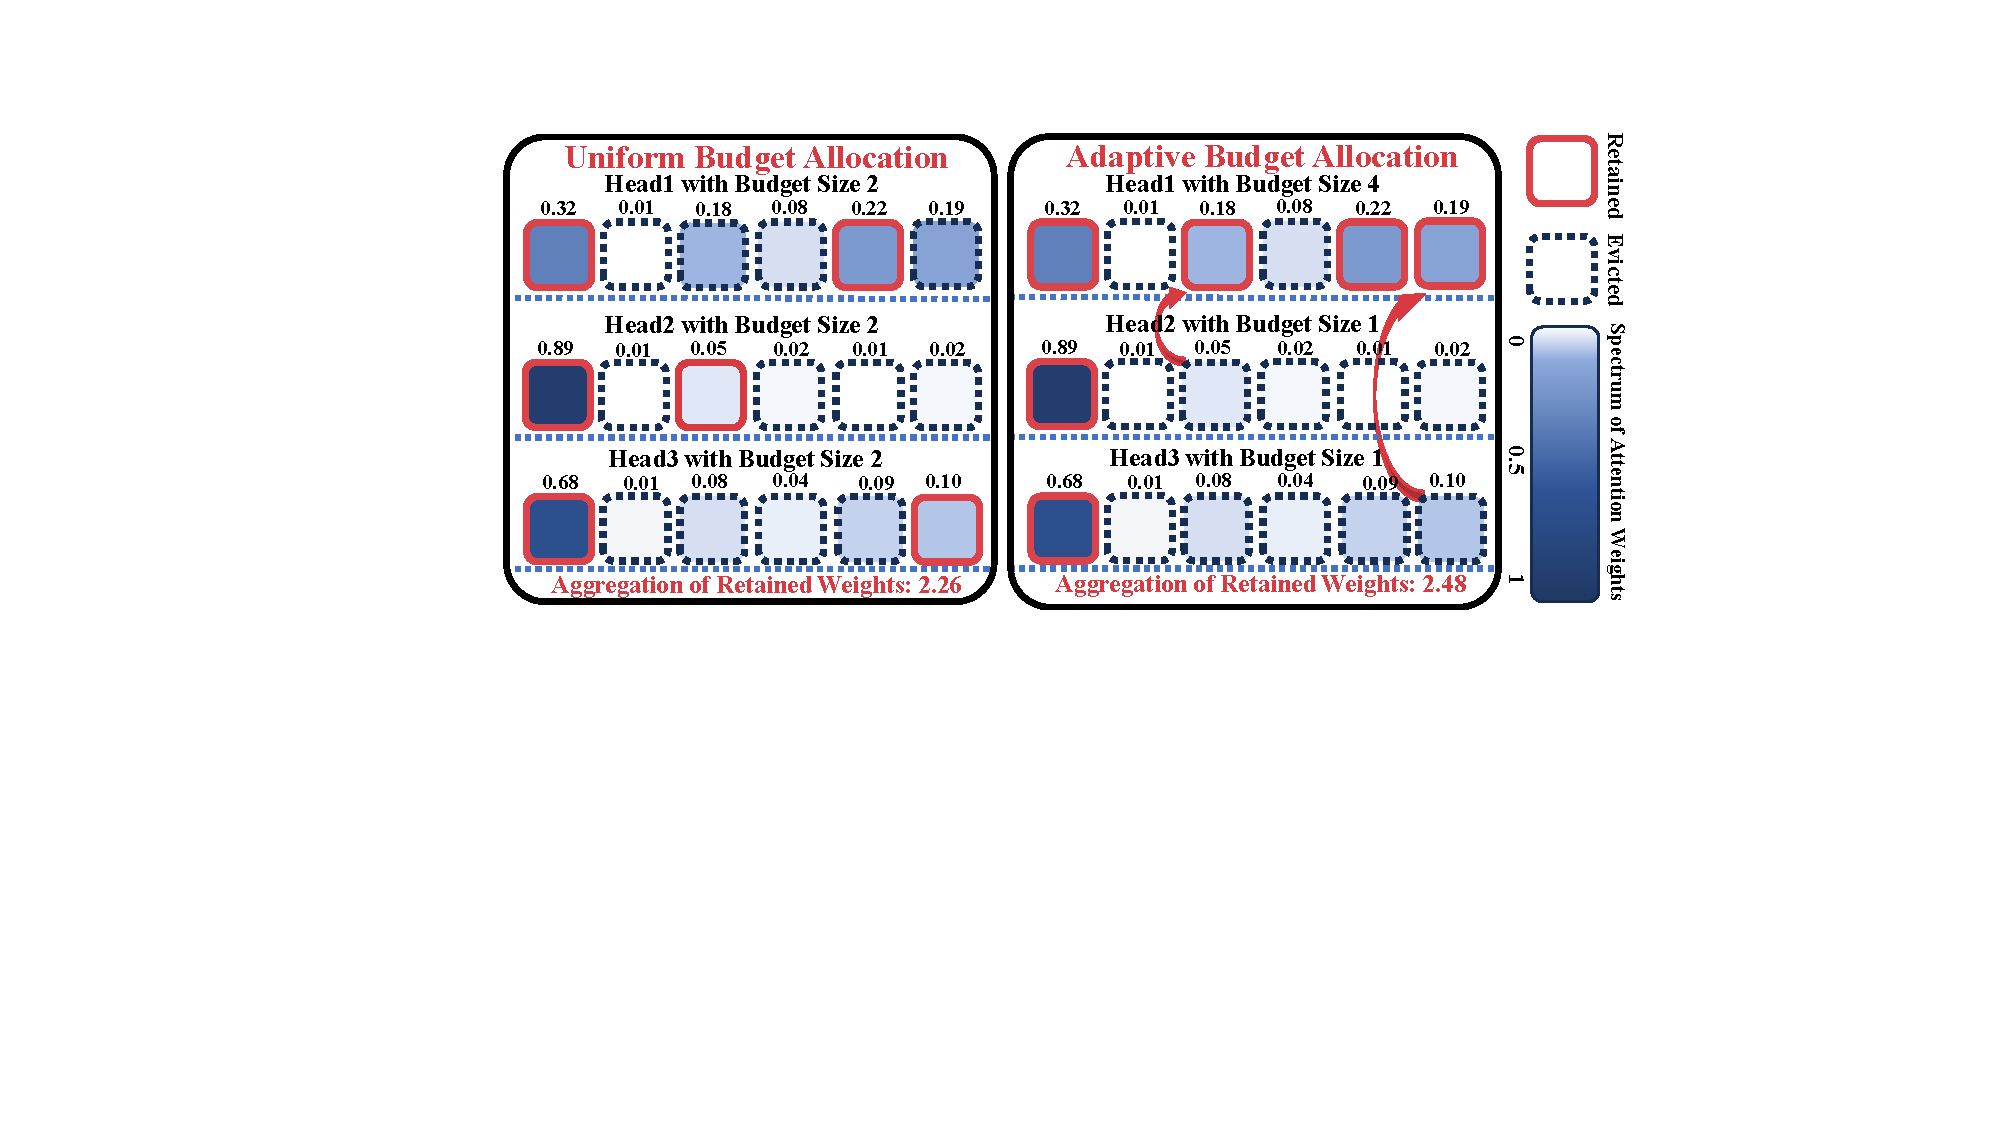
\includegraphics[width=\linewidth]{./Figures/AdaFrame.pdf}
		\vspace{-0.4cm}
		\caption{From Uniform to Adaptive Budget Allocation}
		\label{fig:illu}  
	\end{subfigure}
	\vspace{-0.1cm}
	\caption{Adaptive budget allocation accommodates varying attention concentration across heads. \textit{Left: Analysis using Llama-3.1-8B-Instruct shows most heads retain nearly all attention weights with a small cache (e.g., top 5\%), while dispersed heads require larger cache proportions. Right: Adaptive allocation, which shifts budgets from sparse to dispersed heads, increases the aggregated retained attention weights (from 2.26 to 2.48) and reduces eviction loss compared to uniform allocation.}  
	}  
	\vspace{-0.3cm}
\end{figure}  


However, existing methods uniformly allocate cache budgets across attention failing to account for the unique characteristics of each head.
As shown in Figure~\ref{fig:accu_weights}, attention heads exhibit diverse concentration patterns: some focus narrowly (or sparsely) on a small portion of the cache, while others distribute their attention more broadly \footnote{More visualizations can be found in Appendix~\ref{apdx:heads}}.
This uniform allocation results in inefficiencies---either wasting cache budgets on heads with sparse concentration or incurring significant eviction losses in heads with dispersed distribution. Such imbalances degrade the trade-off between overall budget utilization and the quality of post-eviction generation.
To address this issue, we analyze the impact of existing Top-$k$ eviction methods on attention outputs and propose the first adaptive budget allocation strategy, called {\it Ada-KV}, as illustrated in Figure~\ref{fig:illu}. This strategy dynamically reallocates budgets from heads with sparse concentration to those with more dispersed attention, improving the quality of post-eviction generation.


Our study begins by revisiting Top-$k$ eviction methods, demonstrating that, under specific budget allocation, these methods are equivalent to minimizing an upper bound of eviction loss between pre- and post-eviction attention outputs\footnote{For simplicity, we use $L_1$
  distance to quantify eviction loss; extensions to $L_p$
  norms are possible but orthogonal to this work.}. Based on this, we propose Ada-KV, a simple yet effective adaptive allocation strategy designed to integrate and enhance existing Top-$k$ eviction methods in a plug-and-play manner.
Guided by minimizing the theoretical upper bound of eviction loss, Ada-KV adapts to the varying concentration patterns across attention heads, significantly reducing practical eviction loss.


By integrating the Ada-KV into two state-of-the-art (SOTA) methods, SnapKV \cite{SnapKV} and Pyramid~\cite{PyramidInfer,PyramidKV}, we have developed two integration cases: {\it Ada-SnapKV} and {\it Ada-Pyramid} 
\footnote{
	 The plug-and-play nature of Ada-KV enables broad applicability to existing methods and future developments, extending well beyond the two cases presented in this paper. Section~\ref{sc:broad} provides further examples of its adoption in subsequent work.}.
These methods are evaluated using two comprehensive benchmarks, Ruler and LongBench, which include 13 and 16 datasets, respectively.
Experimental results demonstrate that Ada-KV could effectively improves performance across various budget settings under the widely studied \textbf{question-aware} compression scenario \cite{SnapKV,PyramidKV,H2o}.
 Furthermore, in the more challenging \textbf{question-agnostic} \cite{kvpress} scenario---where compression is applied without leveraging question-specific information, an important scenario that has been largely overlooked---Ada-KV demonstrates even greater advantages.
The main contributions are summarized as follows.

\begin{itemize}
  \item {\bf Adaptive Budget Allocation.}
  We identify a critical limitation in current KV cache eviction methods: their uniform budget allocation overlooks the unique attention patterns of individual heads. To address this, we propose Ada-KV, the first adaptive budget allocation strategy, which enhances budget utilization across individual heads, leading to more efficient cache eviction methods.

  
  \item {\bf Theoretical Insights.}
  We establish a theoretical framework for cache eviction by defining eviction loss and deriving its upper bound. This framework not only explains the optimization target of prior methods but also guides the design of Ada-KV, enabling principled and adaptive budget allocation.
  
  \item {\bf Empirical Advances.}
  With efficient CUDA kernel implementations, Ada-KV offers plug-and-play compatibility, enabling seamless adoption and performance enhancements in existing methods.
  We evaluate Ada-KV by integrating it into SOTA cache eviction methods, and demonstrate significant improvements across 29 datasets from Ruler and LongBench, all under both question-aware and question-agnostic scenarios.
  
\end{itemize}







